\documentclass[11pt]{article}
\usepackage[utf8]{inputenc}
\usepackage[T1]{fontenc}
\usepackage[french]{babel}
\usepackage{graphicx}
\usepackage{geometry}
\usepackage{amsmath}
\usepackage{enumitem}
\usepackage{xcolor}
\usepackage{float}
\usepackage{mdframed}
\usepackage{listings}
\usepackage{xcolor}
\usepackage{ulem}
\usepackage{soul}

\definecolor{codebackground}{rgb}{0.95,0.95,0.95}

\lstdefinestyle{terminal}{
  backgroundcolor=\color{codebackground},
  basicstyle=\ttfamily\small,
  frame=none,
  breaklines=true,
  columns=fullflexible,
  postbreak=\mbox{\textcolor{red}{$\hookrightarrow$}\space},
  showstringspaces=false,
  captionpos=b,
  escapeinside={(*@}{@*)},
  numbers=left,
  numberstyle=\tiny,
  numbersep=5pt
}

\geometry{hmargin=2.5cm,vmargin=1.5cm}

\title{\textbf{Rapport Projet d'introduction à la recherche}}
\author{Aurand-Augier Mathias}
\date{}

\begin{document}

\maketitle
\tableofcontents
\newpage

% \section{Préambule : rappel de l'environnement de travail}

% \vspace{5mm}

% Après s'être connecté sur le serveur, on voit une multitude d'entité sur notre topologie.
% On peut voir en effet : 
% \begin{itemize}[label=\textbullet, leftmargin=1.5cm]
%     \item \textbf{Topologie Gate} : C'est la grosse planète en haut. C'est elle qui connecte notre petit réseau local à Internet, permettant ainsi la communication externe. C'est grâce à ca que quand on se connecte à la machine, on a internet, sinon, on aurait pas de WIFI.
%     \item \textbf{Passerelle / Pare-feu (pfsense)} : C'est le truc orange. C est est un pare-feu et routeur open-source. Il sert à sécuriser le réseau en contrôlant le trafic entrant et sortant selon des règles définies. Il agit également comme passerelle entre le réseau local et Internet. C'est une sorte de portail, ca permet la sécurité. Il joue aussi le role de routeur.
%     \item \textbf{Un serveur Linux}
%     \item \textbf{Un client Linux}
% \end{itemize}

% \vspace{5mm}

% Pour demarrer les machines, on les instancie dans un premier temps en cliquant sur "Definir".
% Puis on le met en mode intelligent, ce qui sert à répartir les charges entre les serveurs de manière intelligente (cela évite la surcharge d'un serveur particulier).
% Ce mode permet une allocation dynamique des ressources en fonction des besoins des VMs (combien de ressources CPU ou de mémoire), de la disponibilité des serveurs, ou même des conditions de réseau.

% % \begin{figure}[H]
% % \centering
% % \includegraphics[width=1\textwidth]{figures/Schema.png}
% % \caption{Schema de la topologie}
% % \end{figure}

% \vspace{5mm}

\section {Motivation}

Considérons un professeur de francais corrigant une rédaction produite par un élève sur un sujet quelconque, comment évalue-t-il la qualité de cette rédaction ? 
Celui-ci dirait surement qu'il se base sur la richesse du vocabulaire, la syntaxe, la cohérence, la pertinence, la clarté, la concision, la précision, la variété des stuctures de phrases, autant de concept relativement 
difficile à mesurer quantitativement et souvent basé sur l'interprétation de chacun. 
Pourtant, la compréhension de ces concepts conditionnent dans une certaine mesure la faculté de l'élève à progresser, comment peut il à l'avenir améliorer sa "cohérence" si la définition du terme n'est pas claire à ses yeux.
En ce sens, remplaçons le professeur par un programme informatique et l'élève par un modèle de langage automatique, comment un programme pourrait il évaluer la qualité d'un texte produit par un autre programme ?
Il faudrait pour cela définir des critères quantitatif de "qualité" d'un texte. 

Une methode possible d'évaluation pourrait se baser sur des références : il ne s'agirait alors pas d'évaluer la qualité d'un texte en lui même, mais plutôt de se demander si un texte semble "de meilleure qualité" qu'un autre.
Pour illustrer ce principe, nous avons à notre disposition 5 générateurs de texte, chacun ayant une qualité de sortie différente. Chaque générateur produit un commentaire relatif à une image donnée.
Le but est de mettre en évidence certains signes de qualités des textes par rapport aux autres.

\section {La notion de "qualité" d'un texte}

\subsection {Richesse du vocabulaire}

Pour évaluer la "qualité" d'un texte, on peut commencer par évaluer la richesse du vocabulaire. 
Par richesse du vocabulaire, on peut entendre plusieurs choses : plusieurs méthodes peuvent être utilisé pour évaluer la richesse du vocabulaire. 
Dans un premier temps, on peut compter le nombre de mots différents généré par chaque intellience artificielle. 

On obtient les résultats suivants : 

\vspace{5mm}

\begin{mdframed}
  \begin{lstlisting}[style=terminal]
    Number of words in BART_1:  433
    Number of words in BART_2:  483
    Number of words in T5_1:  295
    Number of words in T5_2:  310
    Number of words in FST:  194

    Number of words in total:  863  
  \end{lstlisting}
\end{mdframed}

\vspace{5mm}

On peut voir que BART\_2 et BART\_1 ont les plus grands nombres de mots différents, suivi de T5\_2, T5\_1 et FST. Ce qui pourrait être un signe que 
BART\_2 et BART\_1 ont un vocabulaire plus riche que les autres, et qu'elles emploie des mots plus variés. 
Néanmoins, cette méthode n'est pas parfaite, car elle ne prend pas en compte la fréquence d'apparition des mots ni la longueur de la phrase.

Aussi tentons d'évaluer la longueur moyenne des phrases générées par chaque IA. Rien n'affirme que des phrases plus longues sont de meilleure qualité, mais cela pourrait expliquer le nombre de mots différents utilisés. Par ailleurs, 
la longueur de la phrase peut cacher une certaine complexité syntaxique, ainsi qu'un contenu explicatif de l'image commenté mieux fourni : le fond serait alors de meilleur qualité. Voyons ce que ca donne : 

\vspace{5mm}

\begin{mdframed}
  \begin{lstlisting}[style=terminal]
    Average length of sentences in BART_1 : 11.752437914445455
    Average length of sentences in BART_2 : 13.295410219737356
    Average length of sentences in T5_1 : 14.149915485632558
    Average length of sentences in T5_2 : 11.261864516967885
    Average length of sentences in FST : 7.4020283448186195
  \end{lstlisting}
\end{mdframed}

\vspace{5mm}

Les résultats sont très interessant puisque l'on peut voir que T5\_1 a les phrases les plus longues et pourtant un des vocabulaire le plus pauvre, ce qui peut être le signe d'une répétition excessive des mêmes mots. 
Les différences de longueurs entre BART\_1 et BART\_2 sont également interessantes, puisqu'elle pourrait expliquer le différentiel de vocabulaire entre les deux modèles.
Ensuite, la longueur des phrases de FST est la plus faible, ce qui pourrait expliquer la pauvreté du vocabulaire.

Il peut être interessant d'étudier la fréquence d'utilisation des mots les plus fréquents. On peut pour cela utiliser un diagramme à barres empilées (on met ainsi en évidence la contribution de chaque IA à l'utilisation globale de chaque mot).

\vspace{5mm}

\begin{figure}[H]
\centering
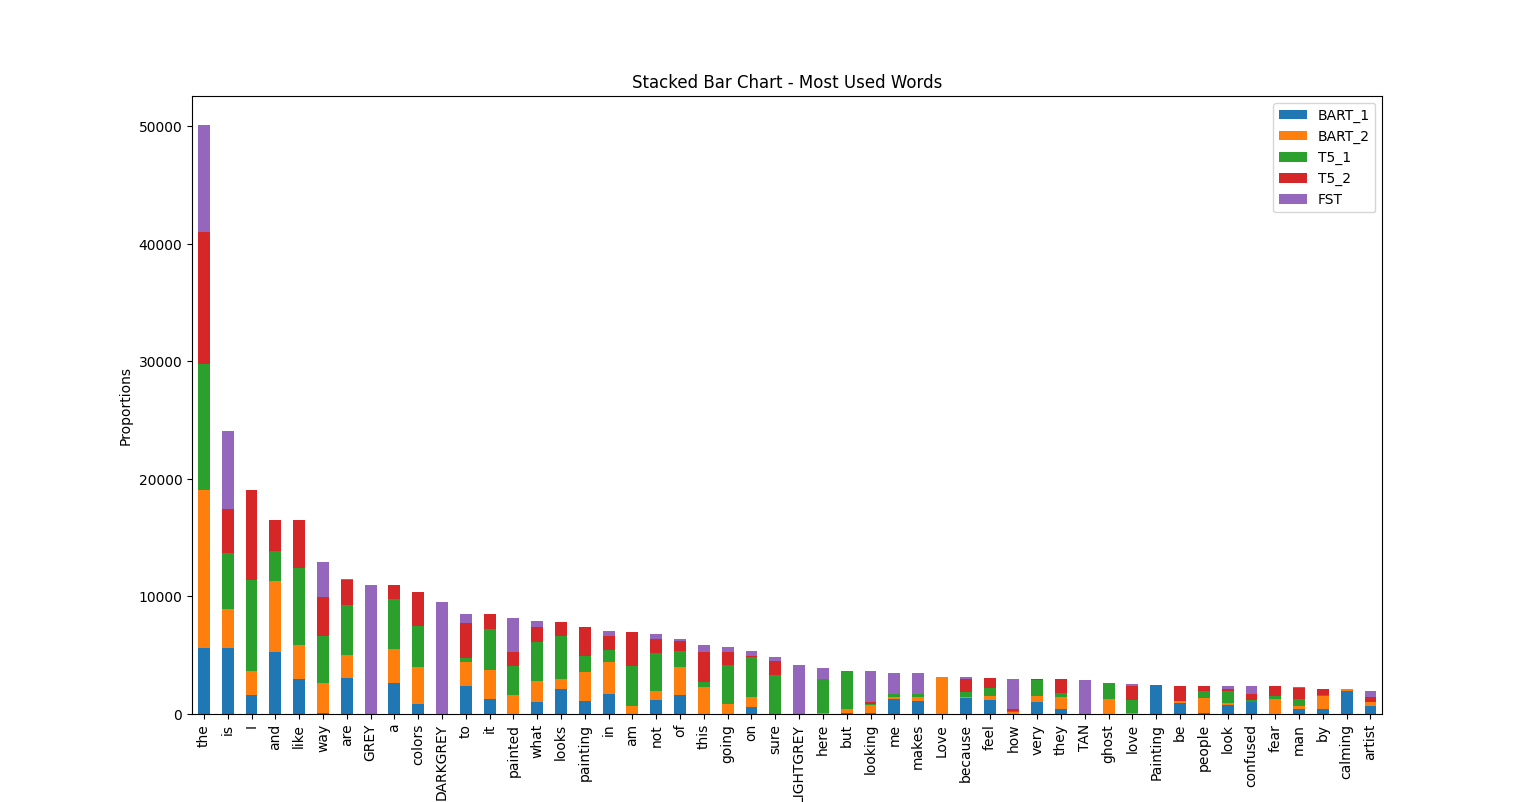
\includegraphics[width=1\textwidth]{../plot/stacked_bars_most_used_words.png}
\caption{Matrice de similarité entre les phrases générées par BART\_1}
\end{figure}

\vspace{5mm}

Un fait particulièrement interessant visible sur ce diagramme est que certains des mots les plus fréquents tel que "grey", "darkgrey", "lightgrey" ne sont utilisé que par FST. Cela révèle une focalisation excessive sur la couleur grise surtout quand on sait que ce n'est pas une couleur si fréquente sur les images. 
La pertinence des réponses de FST peut donc remise en question sachant qu'elle semble concentrée sur les mêmes caractéristiques, cela peut également expliquer la pauvreté du vocabulaire chez FST.

\subsection {Diversité syntaxique au sein d'une même IA}

Une manière interessante de mesurer la capacité d'une intelligence à générer des réponses différentes est de comparer ses propres réponses entre elles : si les phrases sont globalement proche, cela signifie que l'IA a tendance à répéter les mêmes structures de phrases, et donc à manquer de diversité syntaxique.
Voici un exemple : 

\vspace{5mm}

\begin{figure}[H]
\centering
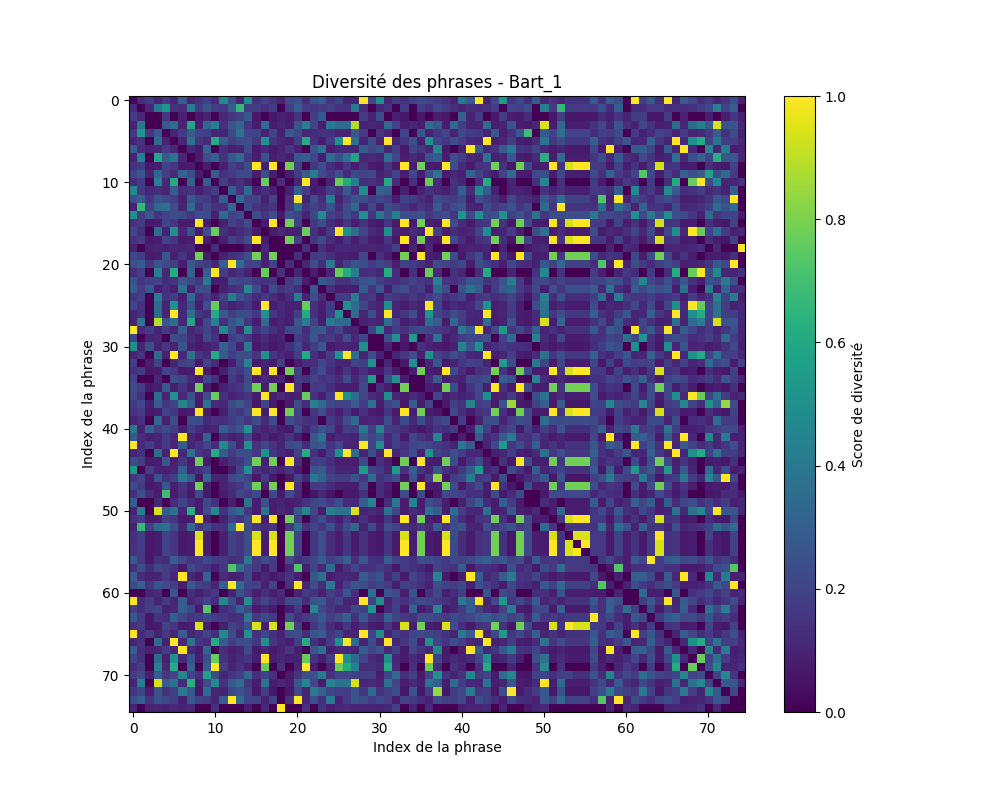
\includegraphics[width=1\textwidth]{../plot/diversity_matrix_bart_1.png}
\caption{Matrice de similarité entre les phrases générées par BART\_1}
\end{figure}

\vspace{5mm}

On remarque ici que la matrice de diversité est relativement sombre, ce qui signifie que les phrases générées par BART\_1 sont relativement différentes les unes des autres, demontrant ainsi une certaine capacité à renouveler les structures.

\vspace{5mm}

\begin{figure}[H]
\centering
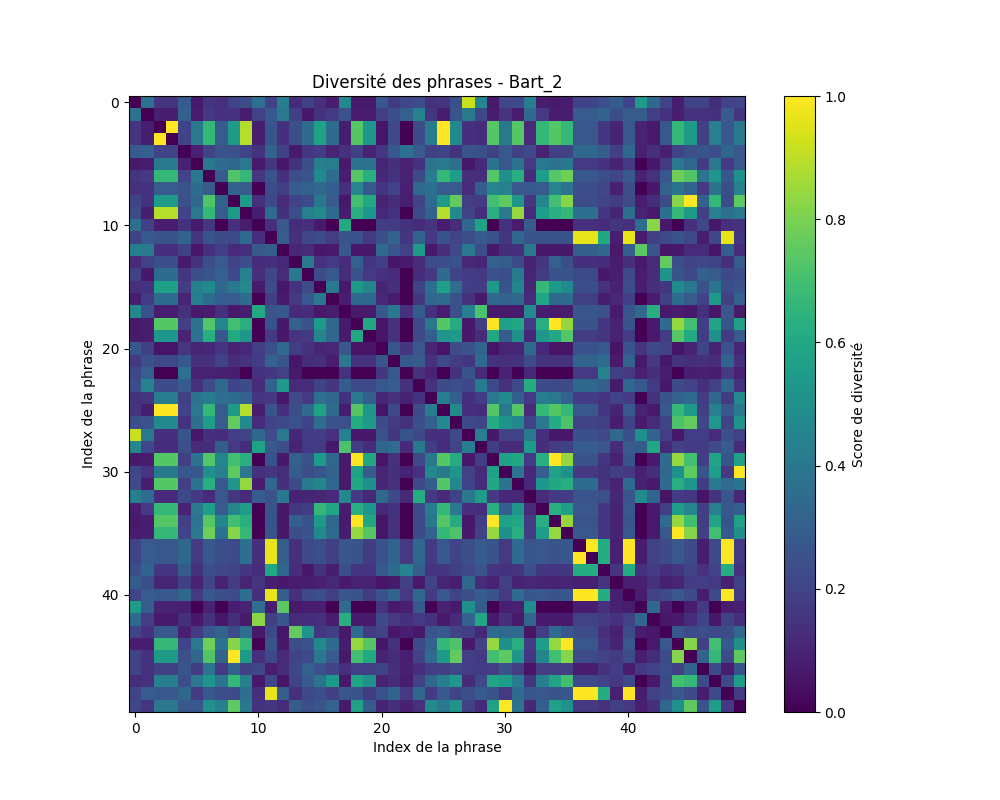
\includegraphics[width=1\textwidth]{../plot/diversity_matrix_bart_2.png}
\caption{Matrice de similarité entre les phrases générées par BART\_2}
\end{figure}

\vspace{5mm}

On remarque ici que la matrice est globalement plus claire que la précédente mais reste néanmoins assez sombre : les phrases sont donc relativement différentes.

\vspace{5mm}

\begin{figure}[H]
\centering
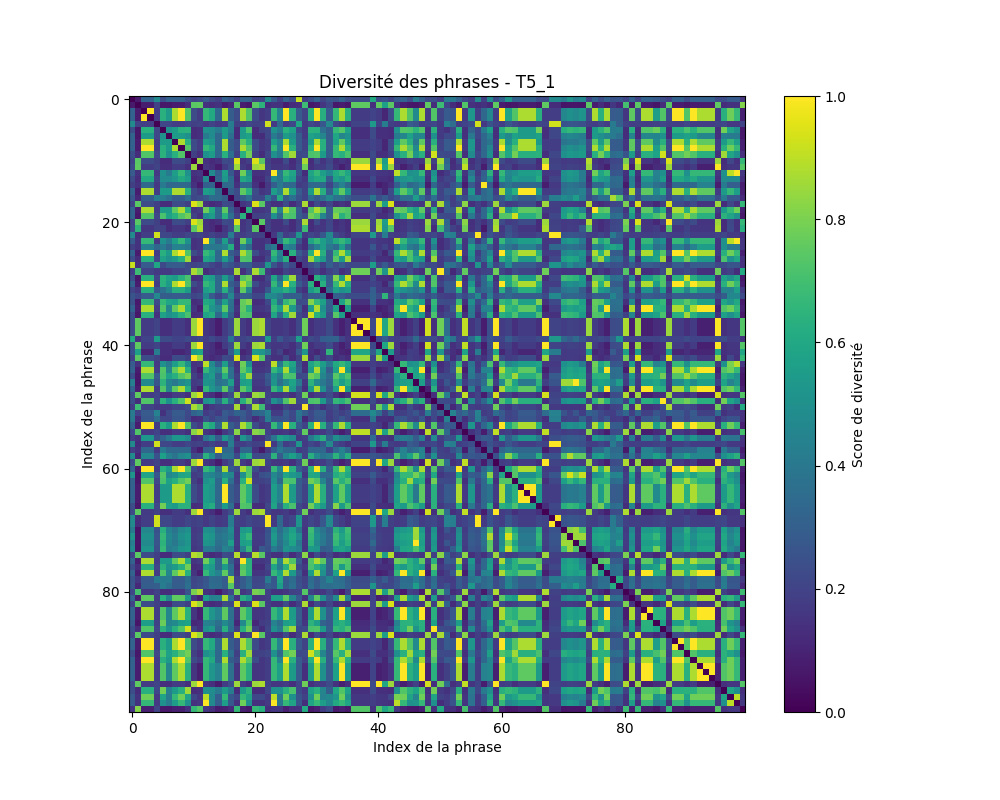
\includegraphics[width=1\textwidth]{../plot/diversity_matrix_t5_1.png}
\caption{Matrice de similarité entre les phrases générées par T5\_1}
\end{figure}

\vspace{5mm}

En revanche, ici il est clair que la matrice a une couleur beaucoup plus claire, ce qui montre que les réponses générées par T5\_1 sont répétitives. Pourtant, quelques points sombres montre qu'elle est capable de se renouveler mais cela semble 
ici ponctuel et non récurrent.

\vspace{5mm}

\begin{figure}[H]
\centering
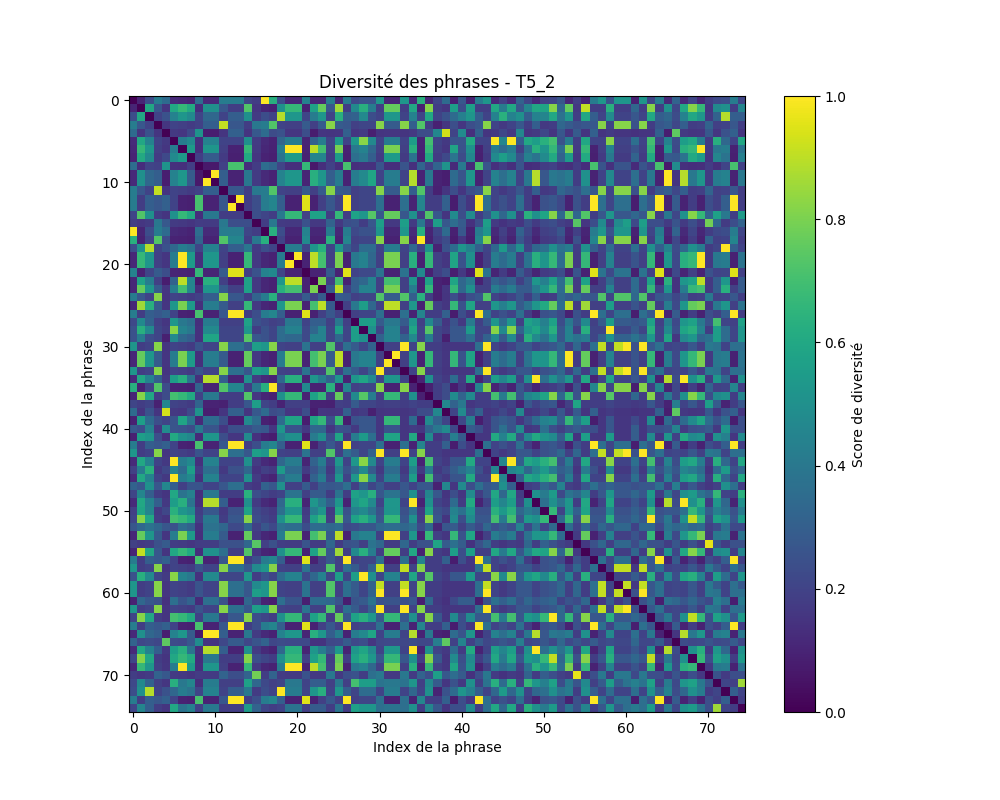
\includegraphics[width=1\textwidth]{../plot/diversity_matrix_t5_2.png}
\caption{Matrice de similarité entre les phrases générées par T5\_2}
\end{figure}

\vspace{5mm}

La matrice de T5\_2 est très similaire à celle de T5\_1, ce qui montre que T5\_2 a également tendance à répéter les mêmes structures de phrases.

\vspace{5mm}

\begin{figure}[H]
\centering
\includegraphics[width=1\textwidth]{../plot/diversity_matrix_fst.png}
\caption{Matrice de similarité entre les phrases générées par FST}
\end{figure}

\vspace{5mm}

De même, la matrice de FST est très similaire à celle de T5\_1 et T5\_2, ce qui montre que FST a également tendance à répéter les mêmes structures de phrases.

\subsection {Mesure de similitude entre les différentes intelligences artificielles}



\subsection {Mesure de similitude au sein des phrases générées par une même IA}
\subsection {}
\subsection {}
\subsection {}

\section {Introduction}





\vspace{5mm}
\end{document}